\section{Classification and Regression Trees}
\subsection{Classification Trees}
$\ct$ is a learning algorithm that can handle binary/Mult-value classificaiton problems with discrete Binary/Mult-value on continus attributs.\\
\textbf{Hypothesis space}:\\
A decision tree is a tree where
\begin{itemize}
    \item Each \textbf{interior nodes} test an attributes
    \item Each \textbf{branch} correspond to an attribute value
    \item Each \textbf{Leaf} node is labelled with a class
\end{itemize}

  \begin{table}[!h]
    \begin{center}
    \begin{tabular}{| m{8em}| m{30em}|}
    \hline
    \centering
    \rowcolor{blue.g} \textbf{Goal}     &  \begin{itemize}
                                              \item Choose a [trees structure/prediciton] model that \textbf{minimize} the \textbf{miss-classification} error  and \textbf{simple}  
                                          \end{itemize}\\ \hline
                                          
    \centering
    \rowcolor{vert.g} \textbf{Optimal}     &  \begin{itemize}
                                              \item Simple \& cohérent avec le LS
                                          \end{itemize}\\ \hline
                                                                                
    \end{tabular}
    \end{center}
    \end{table}

Some $\example$:
\begin{figure}[H]
    \centering
    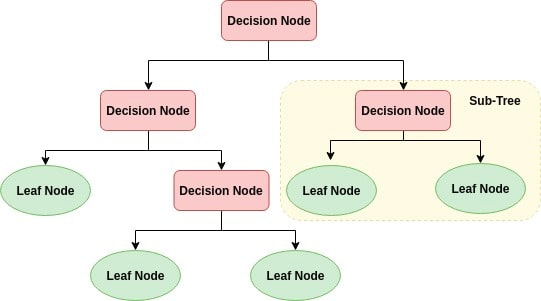
\includegraphics[scale = 0.5]{Question6/DT.jpg}
    \caption{$\Dt$ 1}
    \label{fig:my_label}
\end{figure}
\begin{figure}[H]
    \centering
    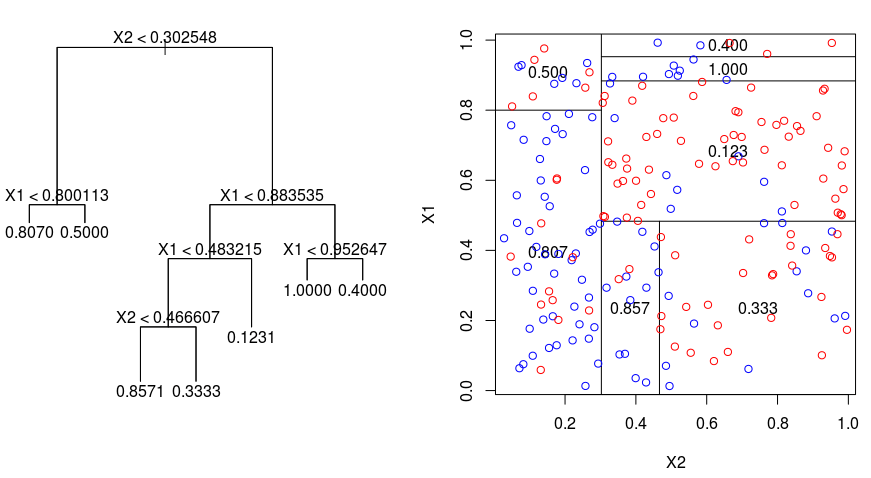
\includegraphics[scale = 0.5]{Question6/DT1.png}
    \caption{$\Dt$ 2}
    \label{fig:my_label}
\end{figure}
\begin{figure}[H]
    \centering
    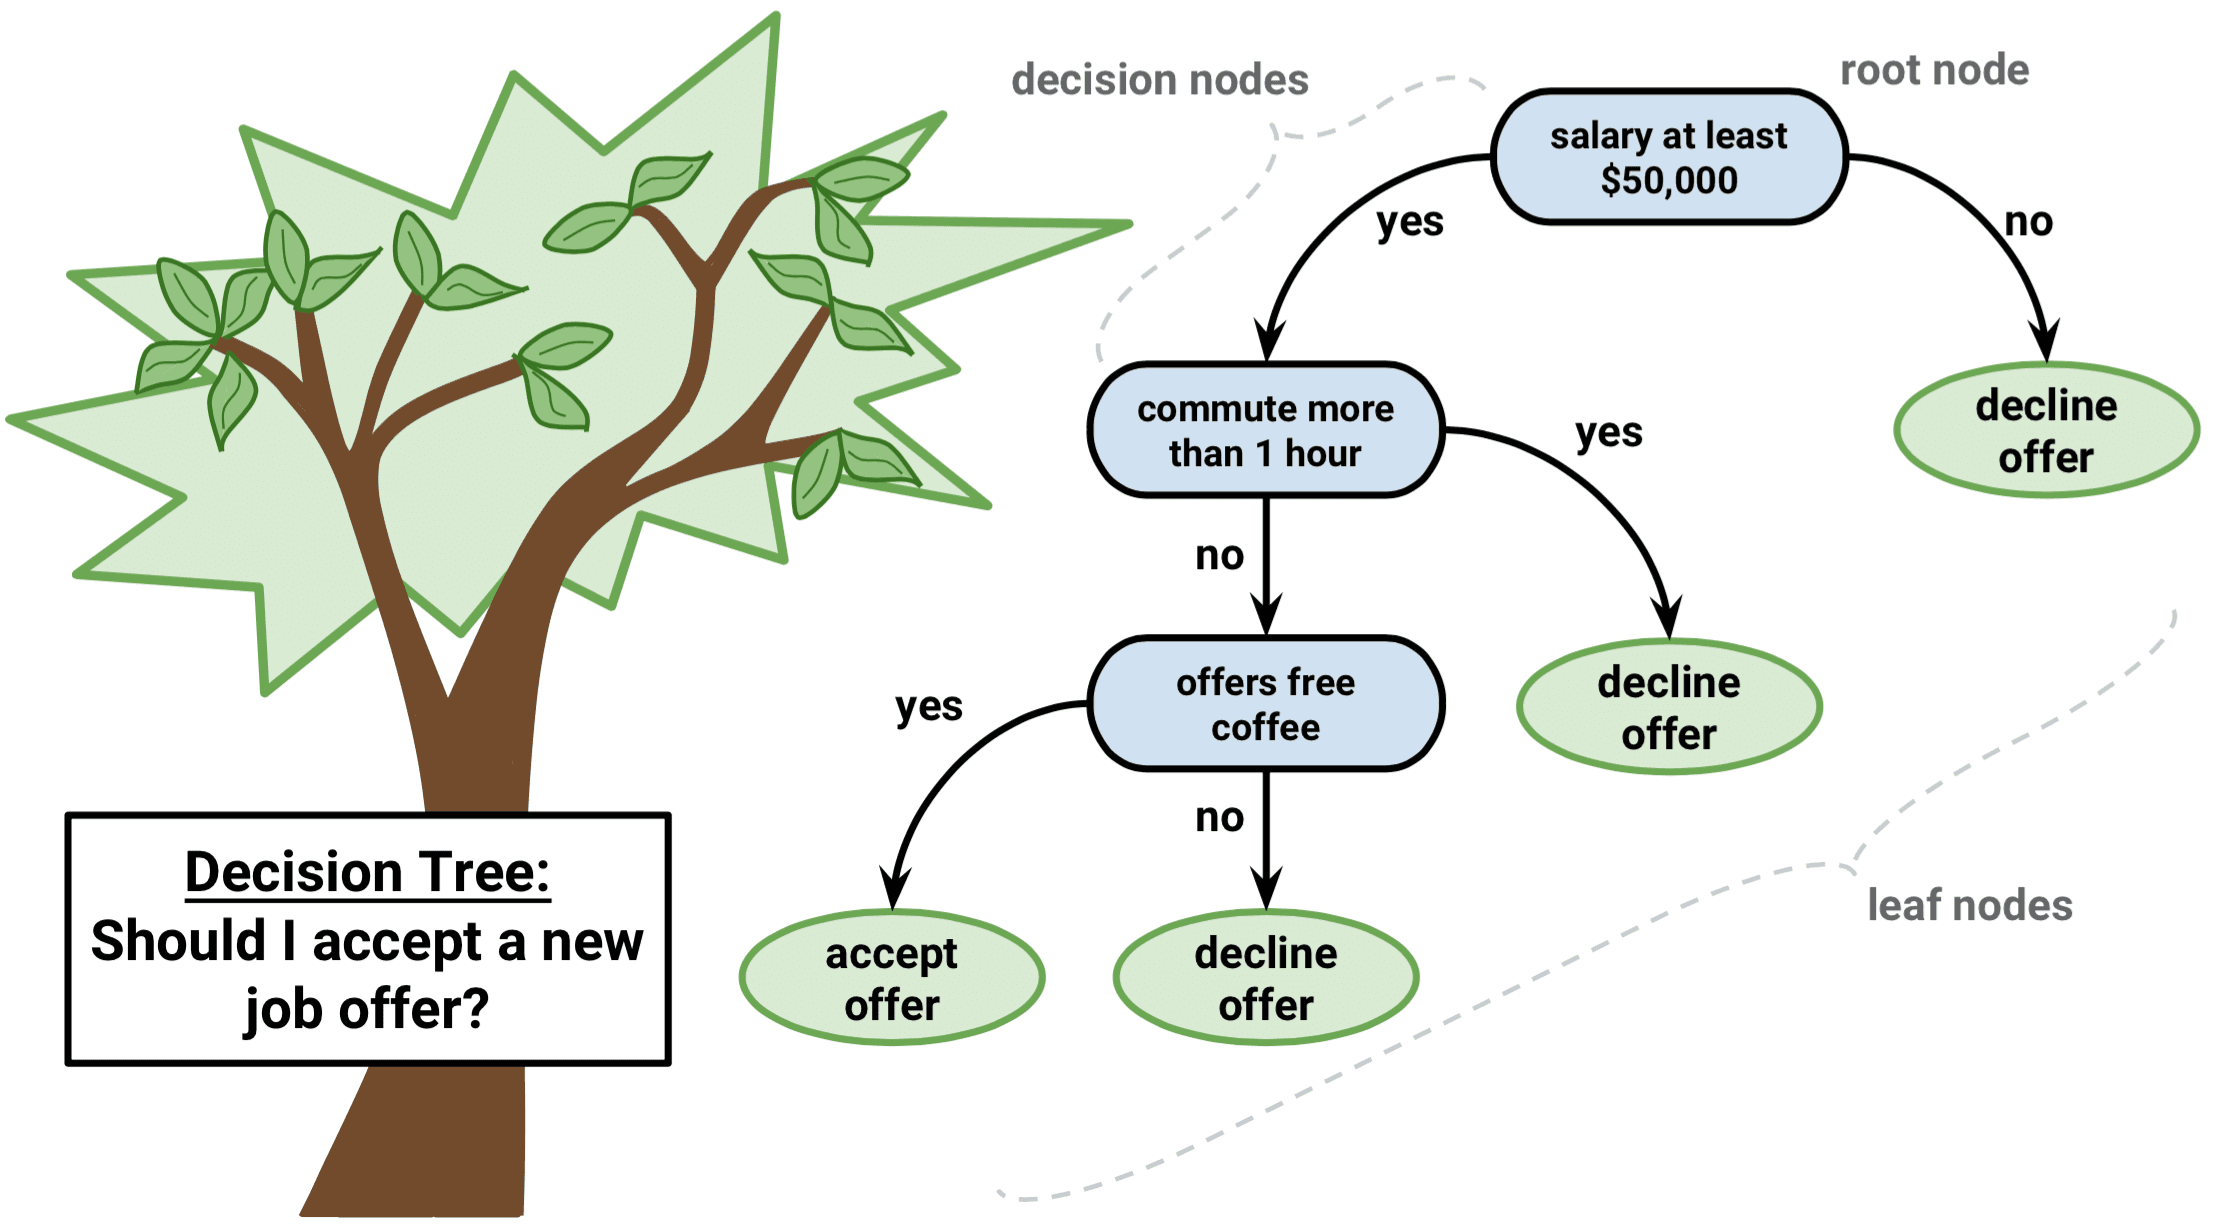
\includegraphics[scale = 0.2]{Question6/DT2.png}
    \caption{$\Dt$ 3}
    \label{fig:my_label}
\end{figure}
%---------------------------- Top-down introduction of DTs -----------------------------------
\subsection{Top-down introduction of DTs}

  \begin{table}[H]
    \begin{center}
    \begin{tabular}{| m{8em}| m{30em}|}
    \hline
    \centering
    \rowcolor{blue.g} \textbf{Method}     &  \begin{enumerate}
                                                \item Choose"Best" attribute
                                                \item Split the LS according to this attribute
                                                \item Proceed Recurcively until each object is correctely classified
                                            \end{enumerate} \\\hline    
    \centering
    \rowcolor{vert.g} \textbf{Properties}     &  \begin{enumerate}
    \item  \textbf{Fast} but \textbf{sub-optimal}
    \item Highly dependent on attribute selection criteria
    \item Hill-climbing algotithm in the space of possible $\dt$ $\rightarrow$ No backtracks \textcolor{red}{simply add sub-trees to current trees}
\end{enumerate}\\ \hline
                                                                                
    \end{tabular}
    \end{center}
    \end{table}
    
Let's define an"impurity measure" I(LS) such that
\begin{enumerate}
    \item I(LS) is \textbf{minimun} if $p_i=1 $ and $p_j=0$, $\forall i \ne j$
    \item I(LS) is \textbf{maximun} if $p_j = \frac{1}{j}$
    \item I(LS) is \textbf{symmetric} with respect to $p_1,..p_j$
\end{enumerate}
The reduction of impurity induced by a split 

  \begin{table}[H]
    \begin{center}
    \begin{tabular}{| m{8em}| m{30em}|}
    \hline
    \centering
    \rowcolor{blue.g} \textbf{Impurity}     &  \begin{itemize}
                                                \item $\Delta I(LS,A) = I(LS) - \sum_a \frac{|LS_a|}{LS}I(LS_a)$
                                                \item $\Delta I$ is the "score measure" (the quantity to \textbf{maximize})
                                                \end{itemize} \\\hline    
    \centering
     \rowcolor{vert.g} \textbf{Impurity}     &  \begin{itemize}
                                                 \item Shannon entropy
                                                 \item Gini Index
                                                 \item Missclass error rate
                                            \end{itemize} \\\hline    
                                                                                
    \end{tabular}
    \end{center}
    \end{table}
    
Used by the CART (classification and regression tree) algorithm for classification trees, Gini impurity is a measure of how often a randomly chosen element from the set would be incorrectly labeled if it was randomly labeled according to the distribution of labels in the subset. The Gini impurity can be computed by summing the probability 
$p_{i}$ of an item with label 
i being chosen times the probability 
$\sum _{k\neq i}p_{k}=1-p_{i}$ of a mistake in categorizing that item. It reaches its minimum (zero) when all cases in the node fall into a single target category.

\subsection{Pré-prunning}
Le pré-prunning stoppe la croissance de l'arbre avant qu'il ne le classifie parfaitement le LS. Arrêter de scinder un noeud si le nombre d'objets est trop petit, si l'impureté est suffisamment faible ou si le meilleur test n'est pas stastiquement significatif.\\
\textbf{Stop condiiton}:
\begin{enumerate}
    \item Nb of objects is too small to split
    \item Imputrity is low enough
\end{enumerate}

%--------------------------- post-prunning ---------------------------------------------------
\subsection{Post-pruning}

\begin{enumerate}
    \item Scinder le LS en deux: GS(growing sample) pour construire l'arbre et \textbf{VS}(calidation sample) 
    pour évaluer son erreur de généralisation. 
    \item Construire un arbre avec GS.
    \item Calculer une séquance d'arbres ${T_1,T_2,..,T_{i-1},T{i},...}$ où T\_i es obtenu en supprimant certains noeuds test de $T_{i-1}$.
    \begin{itemize}
        \item A chaque étape, supprimer le noeud qui diminue le plus l'erreur sur VS.
        \item Définir un critère de coût-complexité et construire la séquance d'arbres qui minimisent le critère.
    \end{itemize}
    \item Sélectionner le $T_i$ qui minimise l'erreur sur le \textbf{VS}
\end{enumerate}
%--------------------------- Tree sequence constructive --------------------------------
\subsection{Tree sequence constructive}
\textbf{2 methodes:}
\begin{enumerate}
    \item \textbf{Reduce error prunning}: \begin{itemize}
        \item at each step, remove the node that most decrease the error on \textbf{LS}
    \end{itemize}
    \item \textbf{Cost-complexity Prunning}
    \begin{itemize}
        \item Define Cost-complexity criteria : $$\textrm{Error}_{GS} + \alpha.\textrm{ complexity}(T)$$
        \item Build the sequence that minimizes this criteria for groing "$\alpha$"
    \end{itemize}
    \textcolor{ao}{ If small DB, use N-fold cross validation}
\end{enumerate}
%--------------------------- Continuous attributes -------------------------------------
\subsection{Continuous attributes}
\textbf{2 solutions:}

  \begin{table}[H]
    \begin{center}
    \begin{tabular}{|m{20em}|}
    \hline
    \rowcolor{blue.g} \textbf{Pre-discretation}\\ \hline
    \rowcolor{vert.g} \textbf{Discretize while tree growth}            
    \end{tabular}
    \end{center}
\end{table}


In addition to find the best attribute, you will also need to find the best cut-point where to discretize. \textcolor{red}{Use of impurity measure as well}
%--------------------------- Multi-value Attributes -------------------------------------
\subsection{Multi-value Attributes}

 2 solutions:
  \begin{table}[H]
    \begin{center}
    \begin{tabular}{|m{20em}|m{20em}|}
    \hline
    \rowcolor{blue.g} \textbf{Penalized attributes with several values} & To avoid data fragmentation too quick caused by multi-value attributes\\ \hline
    \rowcolor{vert.g} \textbf{Consider binary spits} &           
    \end{tabular}
    \end{center}
\end{table}
 But for "\textbf{N}" values attributes $\rightarrow 2^{N-1}$ possible split.\\
 \textcolor{red}{heurishcs if N  "$>>$"}

%--------------------------- Regressions TREE ----------------------------------------------
\subsection{Regression Trees}
Learning algorithm that will handle regression problems (real outputs) with real/discrete attributes.\\
\textbf{Hypothesis space}:\begin{itemize}
    \item similar to class $\dt$\\
    \textcolor{red}{but} leaf nodes are labelled whith a real NB.
\end{itemize} 

\textbf{Tree concstruction}

  \begin{table}[H]
    \begin{center}
    \begin{tabular}{|m{20em}|m{20em}|}
    \hline
    \rowcolor{blue.g} \textbf{Methods} & \begin{enumerate}
    \item Prediction at a leaf 
    \item Impurity of sample:\textbf{ $I(LS) = var_{y|LS}\{y\}$}
    \item best split: split reducing the most the $\variance$
\end{enumerate}\\ \hline
    \rowcolor{vert.g} \textbf{Prunning \algo} &    \begin{enumerate}
    \item pre-prunning : same
    \item post-prunning: use of mean squared error as quality measure
\end{enumerate}       
    \end{tabular}
    \end{center}
\end{table}


\subsubsection{Interpret ability}
DT are ofen used to pre-processed LS to avoid irrelevant varibles as it's a model with a very good/clean visualization of the relatin bwt inputs and outputs

\subsubsection{Advantages/Drawbacks}
  \begin{table}[H]
    \begin{center}
    \begin{tabular}{|m{20em}|m{20em}|}
    \hline
    \rowcolor{vert.g} \textbf{Advantages} & \begin{enumerate}
    \item Fast: $(n\log n)$ 
    \item flexible
\end{enumerate}\\ \hline
    \rowcolor{red.g} \textbf{Drawbacks} &    \begin{enumerate}
    \item Tree instability \textbf{Hight variance} (overfit quickly)
    \item not accuracy
\end{enumerate}       
    \end{tabular}
    \end{center}
\end{table}
